\documentclass[twocolumn]{IEEEtran}
\usepackage{graphicx}
\usepackage{subcaption}
\usepackage{hyperref}

\begin{document}
\title{Acercamiento a la Solucion del Agente Viajero con el uso de Algoritmos Genéticos}
\author{Angel David Corredor}
\date{}
\maketitle

\begin{abstract}
    El artículo presenta una técnica para resolver el problema clasico del Agente Viajero
    (Traveling Salesman Problem) mediante algoritmos evolutivos. El algoritmo es aplicado en
    algunos de los problemas incluidos en la TSPLibrary y sus resultados contrastados con el ya
    popular algoritmo de Ascenso a la Colina.     
\end{abstract}

\section{Introducción}

El problema del agente viajero es uno de los los problemas clasicos de optimizacion NP-hard.
En este problema se tienen $n$ ciudades y las distancias entre ellas estan dadas por una matriz
$D=d_{ij}$ ($d_{ij}$, la distancia entre las ciudades $i$ y $j$).
Tenemos un vendedor que debe visitar cada una de las ciudades exactamente una vez. Se asume que 
su velocidad de desplazamiento es constante ($v_c$) e intenta minimizar el tiempo que toma completar
el tour.
La funcion objectivo se define entonces como:

\begin{equation}
    f(\bar{x}) =
    \sum_{i=1}^{n-1} (t_{x_i,x_{i+1}})
    + t_{x_n,x_1},
    \bar{x}=(x_1,...,x_n)
\end{equation}

donde $\bar{x}$ representa un tour, el cual contiene cada una de las ciudades exactamente una vez
y $t_{x_i,x_{i+1}}$ es el tiempo de viaje entre $x_i$ y $x_{i+1}$ el cual se calcula como:

\begin{equation}
    t_{x_i,x_{i+1}} =
    \frac{d_{x_i,x_{i+1}}}{v_c}
\end{equation}

Claramente, $f$ es el tiempo total que toma completar el tour.
El objetivo es entonces encontrar el $\bar{x}$ que minimiza $f$. 

\section{Representacion y Operadores}

De manera tradicional los individuos para TSP son representados como una permutación de $n$
elementos llamado tour, la cual representa el orden en el que el vendedor debe visitar
cada una de las ciudades.

Una vez definida una representación adecuada, se proceden a elegir los operadores geneticos que
serán usados sobre estos individuos, los cuales son:

\subsection{Mutación}
La mutación es un operador unario el cual modifica una parte del código genetico, el operador
seleccionado toma aleatoriamente 2 elementos del genoma y los intercambia, manteniendo de esta
forma una permutación valida. 

\subsection{Cruce}
El cruce es un operador binario el cual utiliza 2 individuos que se toman el rol de "padres",
los cuales combinan su genoma de manera que se obtienen 2 nuevos individuos "hijos".
El operador usado selecciona una posicion aleatoria del genoma de un copiando los elementos 
a uno de los hijos, los elementos que hacen falta para completar el tour se toman 
del otro padre segun el orden que tengan en el genoma de este. D esta forma se preserva parte de
la nformación de ambos caminos. Para el segundo hijo se procede de igual manera pero cambiando
el orden de los padres.

\section{Algoritmo Propuesto}

El algoritmo usado para la resolución del problema del Agente Viajero es un Algoritmo Genético
de estado estable con una selección de padres uniforme y una probabilidad de cruce de 0.7 
por cada pareja de padres. Como operadores de mutación y cruce se utilizan los anteriormente expuestos.

Este algoritmo al ser de estado estable asegura que se mantiene la mejor solución hallada a travez
de las generaciones a la vez que los operadores presentados en la sección previa permiten hacer una
exploración mas amplia del espacio de busqueda.

\section{Resultados}

Para los experimentos se usaron los problemas bays29, eil51 y d198 de la TSPLib,
posteriormente se compara el rendimiento estadistico de la técnica comparada con Ascenso a 
la Colina Paralelo el cual implementa unicamente mismo el operador de mutación.
Para cada experimento se hicieron 30 ejecuciones independientes del algoritmo, 
contando cada una de ellas con 100 generaciones de 100 individuos cada una.
\\
El código empleado se puede encontar en \url{https://github.com/adcorredorm/Evolutionary_Computing}
\\

Los resultados obtenidos fueron:

\begin{figure}
    \centering
    \begin{subfigure}[b]{1\linewidth}
        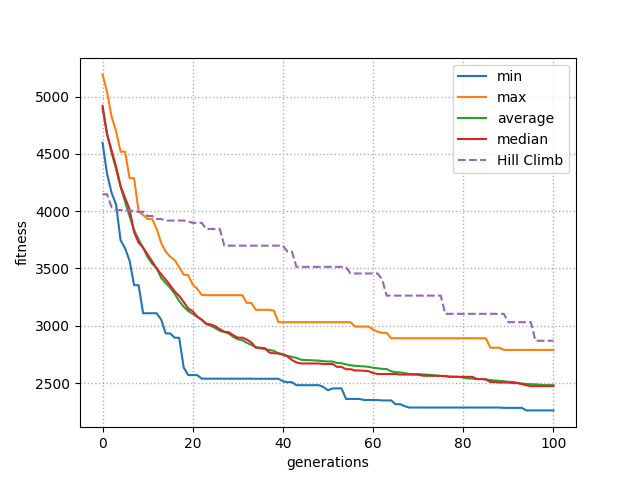
\includegraphics[width=\linewidth]{figures/tsp29.png}
        \caption{Resultados bays29}
    \end{subfigure}
    \begin{subfigure}[b]{1\linewidth}
        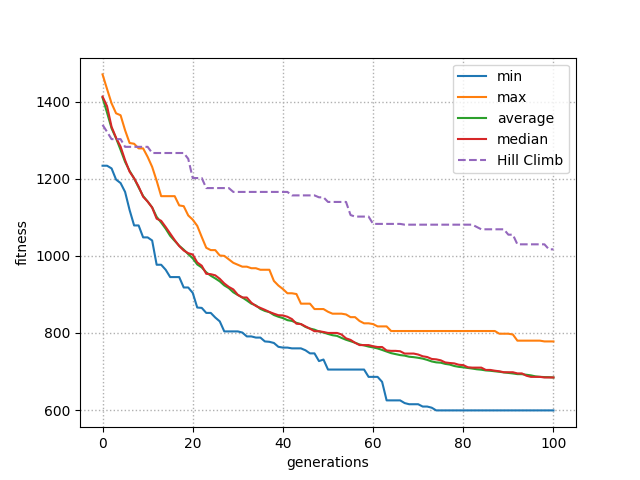
\includegraphics[width=\linewidth]{figures/tsp_51.png}
        \caption{Resultados eil51}
    \end{subfigure}
    \begin{subfigure}[b]{1\linewidth}
        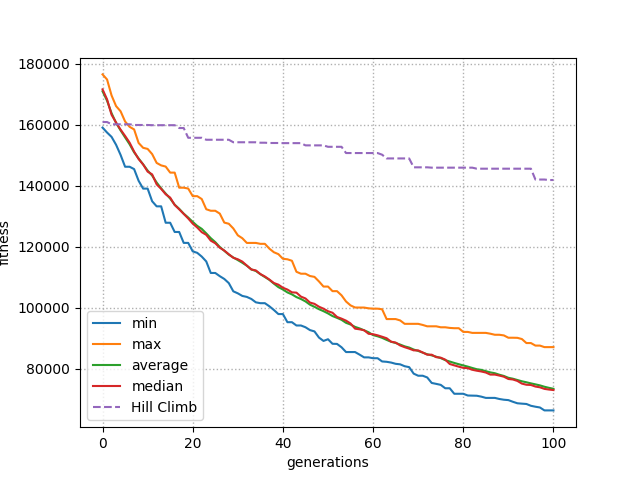
\includegraphics[width=\linewidth]{figures/tspd198.png}
        \caption{Resultados d198}
    \end{subfigure}
    \caption{Resultados Algoritmo Genetico V.S Ascenso a la Colina}
\end{figure}

\begin{table}[htpb]
\centering
\begin{tabular}{|c|c|c|c|c|}
    \hline
    Problema & $\bar{x}$ & $\sigma_{\bar{x}}$ & mediana & $\sigma_{med}$ \\
    \hline
    bays29 & 2481.7 & 135.437 & 2472.5 & 135.7599 \\
    \hline
    eil51 & 684.4 & 43.9526 & 684.5 & 43.9528 \\
    \hline
    d198 & 73410.8667 & 3899.324 & 72993.5 & 3922.3628 \\
    \hline
\end{tabular}
\caption{Resumen estadistico algoritmo genético por problema}
\label{table:results_ga}
\end{table}

\begin{table}[htpb]
    \centering
    \begin{tabular}{|c|c|c|c|c|}
        \hline
        Problema & $\bar{x}$ & $\sigma_{\bar{x}}$ & mediana & $\sigma_{med}$ \\
        \hline
        bays29 & 3320.1 & 131.7648 & 3349.5 & 135.1152 \\
        \hline
        eil51 & 1077.1667 & 30.2405 & 1071.5 & 30.7848 \\
        \hline
        d198 & 150738.8 & 3776.984 & 151105 & 3795.3043 \\
        \hline
    \end{tabular}
    \caption{Resumen estadistico ascenso a la colina por problema}
    \label{table:results_hc}
    \end{table}

\section{Conclusiones}

Como se puede observar en la tabla \ref{table:results_ga} y \ref{table:results_hc}, el algoritmo
genetico supera ampliamente al ascenso a la colina, lo cual se puede comprobar rapidamente 
haciendo una prueba de hipotesis sobre los valores de la media o la mediana de ambos algoritmos.
Por tanto el algoritmo genetico aqui propuesto es viable para dar solucion al problema del
agente viajero.

\begin{thebibliography}{X}
    \item Bonyadi, Michalewicz, Barone. The travelling thief problem: the first step in the
    transition from theoretical problems to realistic problems. \url{https://cs.adelaide.edu.au/~zbyszek/Papers/TTP.pdf}  
    \item TSPLib. Travelling Salesman Problem Instances and best known solutions.
    \url{http://elib.zib.de/pub/mp-testdata/tsp/tsplib/tsplib.html}
    \item Rodriguez, Gomez. Solución de problemas tipo Flow-Shop mediante algoritmos evolutivos.
    \url {http://bdigital.unal.edu.co/12916/}
\end{thebibliography}

\end{document}